% 
% Annual Cognitive Science Conference
% Sample LaTeX Paper -- Proceedings Format
% 

% Original : Ashwin Ram (ashwin@cc.gatech.edu)       04/01/1994
% Modified : Johanna Moore (jmoore@cs.pitt.edu)      03/17/1995
% Modified : David Noelle (noelle@ucsd.edu)          03/15/1996
% Modified : Pat Langley (langley@cs.stanford.edu)   01/26/1997
% Latex2e corrections by Ramin Charles Nakisa        01/28/1997 
% Modified : Tina Eliassi-Rad (eliassi@cs.wisc.edu)  01/31/1998
% Modified : Trisha Yannuzzi (trisha@ircs.upenn.edu) 12/28/1999 (in process)
% Modified : Mary Ellen Foster (M.E.Foster@ed.ac.uk) 12/11/2000
% Modified : Ken Forbus                              01/23/2004
% Modified : Eli M. Silk (esilk@pitt.edu)            05/24/2005
% Modified : Niels Taatgen (taatgen@cmu.edu)         10/24/2006
% Modified : David Noelle (dnoelle@ucmerced.edu)     11/19/2014

%% Change "letterpaper" in the following line to "a4paper" if you must.

\documentclass[10pt,letterpaper]{article}

\usepackage{cogsci}
\usepackage{comment}
\usepackage{pslatex}
\usepackage{apacite}
\usepackage{amsmath,amssymb}
\usepackage{graphicx}
\usepackage{subcaption}
\usepackage{color}
\usepackage{url}
\usepackage{todonotes}
\usepackage{mathtools}
\usepackage{stmaryrd}
\usepackage{booktabs}
\usepackage{array}
\usepackage{caption}
\usepackage{subcaption}
\usepackage[export]{adjustbox}


\newcommand{\jefan}[1]{{\color{blue}{[jefan: #1]}}}
\newcommand{\kushin}[1]{{\color{orange}{[kushin: #1]}}}

\title{Semantic structure in communicative drawings}
 
\author{\begin{tabular}[htbp]{c@{\extracolsep{1em}}c@{\extracolsep{1em}}c@{\extracolsep{1em}}c} \\
{\large \bf Kushin Mukherjee} & {\large \bf Robert X. D. Hawkins} & {\large \bf Judith E. Fan}\\
Department of Cognitive Science  & Department of Psychology & Department of Psychology \\ 
Vassar College & Stanford University & Stanford University \\
\texttt{kumukherjee@vassar.edu} & \texttt{rxdh@stanford.edu} & \texttt{jefan@stanford.edu} \\
\end{tabular}
}

\begin{document}

\maketitle 

\begin{abstract}
\jefan{Placeholder abstract: Sets this paper up as being about visual communication, that we use semantic segmentation data to investigate.}
Drawing is a versatile tool for communication, spanning detailed renderings and simple sketches. 
Even the same object can be drawn in different ways, depending on the context. 
How do people decide how to draw in order to be understood?
Here we investigate the semantic structure of drawings as a window into how people deploy both perceptual information and conceptual knowledge to produce communicatively effective drawings in context.
We analyzed a dataset containing drawings of real-world objects that were produced in different semantic contexts, and contained both detailed and simpler sketches of each object. 
We explored the hypothesis that during visual communication, people spontaneously decompose visual objects into semantically meaningful parts (e.g., chairs consist of legs, seat, and back), resulting in a tight correspondence between the organization of this semantic part knowledge and the procedure people use to sketch an object. 
For example, if someone aims to produce a recognizable sketch of a chair, they produce strokes that represent individually meaningful parts, e.g., seat, armrest, legs.
To investigate this, we developed a web-based platform to collect dense semantic annotations of the stroke elements in each drawing. 
We found that: (1) people are highly consistent in how they interpret what individual strokes mean; (2) single strokes tend to represent a single part category (e.g., leg vs. leg + seat), while multiple strokes may be combined to represent an entire part category (e.g., all the legs on a chair); and (3) strokes representing the same part tend to be clustered in time, suggesting that people tend to start and finish drawing one part of an object before moving onto the next.

\textbf{Keywords:} 
sketching; cognitive science; perception
\end{abstract}

\section{Introduction}
This is where our introduction will go.

\section{Methods}

\subsection{Dataset}

We required sketches of common objects created under different contexts. 
So we obtained sketch data from a two-player 'Pictionary'-style reference game experiment. 
In this experiment, a 'sketcher' aimed to produce sketches of target objects to distinguish them from three distractor objects. 
A 'viewer' had to guess which of the 4 images the sketch represented. 
The targets and distractors were chosen from a set 32 real-world objects belonging to 4 basic-level categories: cars, chairs, dogs, and birds. 
Each category had 8 distinct exemplars. 
There were 2 main context conditions in this experiment - close and far. 
In the close condition, the target image and the distractors belonged to the same basic-level category. 
In the far condition, the target and each of the distractors belonged to a different basic-level category.

We obtained 1198 sketches for the annotation task. 
These sketches were represented as scalable vector graphics (SVG) images. 
The strokes that participants made on the canvas when creating the sketch can be represented as a concatenated string of cubic Bezier curves.  
Thus, the final sketch can be represented by a list of such concatenated strings, each of which corresponds to an event of the participant placing their drawing instrument on the canvas, making some marks on the canvas, and lifting the instrument off of the canvas. 
We were interested in collecting fine-grained annotations of these strokes, so we split strokes into sub-stroke elements, which we called splines. 
A single spline was equivalent to a single cubic Bezier curve, i.e., a Bezier curve with two fixed end points and two control points to control curvature. 
We had participants in our annotation task label each sketch's constituent splines.


\subsection{Participants}

We recruited a total of 326 participants via Amazon Mechanical Turk (AMT).  
For this experiment, participants provided informed consent in accordance with the Stanford University IRB. 
Participants were paid a base amount of \$0.35 and were given an additional bonus of \$0.002 for every stroke they annotated. 
In addition to this, they were given a \$0.02 bonus for every sketch for which they labeled all strokes. 

\subsection{Annotation Procedure}

To collect fine-grained annotations of our sketches, we implemented a web-based Javascript annotation tool. 
Each participant annotated 10 sketches. 
We provided participants with a sketch to be annotated on a canvas as well as a category-specific menu of labels, which they were encouraged to use for the annotation task. We also provided them with the option of entering their own labels through a free-response box. 
The original set of images the sketcher had to discriminate between were shown to help the annotator better understand the contents of the sketch.
Labeling was done by clicking on individual splines or clicking and dragging across multiple splines to highlight them before assigning them a label.
Participants were encouraged to conduct their labeling of strokes in bouts — they were to highlight all the strokes corresponding to a single instance of a part before selecting a label from the menu. 
Participants could do the task at their own pace and continue to a subsequent sketch whenever they felt they were ready. 
They could choose to continue to the next trial without labeling every stroke in a sketch, but they would lose out on the completion bonus as well as the amount they would have earned for labeling the remaining strokes.
\noindent In total, we collected 3608 annotations of 1195 unique sketches. 

\subsection{Preprocessing}
After collecting annotations, we filtered out any sketches that weren't fully annotated. This means that any sketch which didn't have all of its constituent splines labeled was excluded. This left us with 3319 annotations of 1190 unique sketches.
Since there was some variability in the number of times each sketch in our dataset was annotated, we selected those sketches that had been annotated exactly 3 times. This left us with 764 unique sketches, each of which had been annotated 3 times.
We also created unique dictionaries for each object category that mapped participant-generated labels to the most frequently occurring labels in our dataset. This helped reduce the total number of unique labels in our dataset from 228 to 24.




\subsection{Analysis}

We were interested in how reliably different people saw the same parts in abstract sketches of objects. So we looked at inter-annotator reliability in spline labels between participants for each spline in our dataset. Reliability was measured in terms of 'agreement' on spline labels. For example, a 3/3 agreement score for a given spline meant that each of the 3 annotators applied the same label to that spline.

While we decided to collect annotation data at the level of splines, it is possible that strokes themselves correspond to individual instances of parts. To assess the relationship between strokes and semantically meaningful parts we investigated 3 possible correspondence relationships — a) Singular strokes correspond to singular parts b) Singular strokes are used to convey multiple parts, that is, strokes cross semantic boundaries c) Multiple strokes are required to convey a single part. We compared a) and b) by looking at within-stroke label agreement for spline labels for all strokes in our dataset. High agreement among all the splines in a given stroke would be indicative of that being used to represent a single part. On the other hand, low agreement would indicate that stroke crosses semantic boundaries and is used to represent different parts.

We also compared b) and c) by looking at the average number of strokes used to represent specific parts within a given category of sketches. A high average number of strokes for a given part would indicate that multiple strokes are utilized to draw that part, whereas a low average would indicate that a single or few strokes might suffice in depicting that part.

To assess whether participants organized their sequences of strokes in terms of semantically meaningful parts, we coded each stroke in our sketches in terms of their part label and calculated 'part-streaks' — streaks of strokes belonging to the same part being drawn successively in sequence. Averaging these part streaks within a sketch gave us an average streak length, which indicated to what extent participants made strokes belonging to the same part in succession. Next, we scrambled the order of strokes within sketches and calculated the average streak length again. We took the difference between the true average streak length and scrambled average streak length and repeated this processes several times to obtain a sampling distribution of the difference between the true and scrambled streak lengths. 

\section{Results}
\subsection{Inter-annotator reliability}
67.85\% of splines in our dataset had 3/3 inter-annotator agreement, 27.77\% of splines had 2/3 agreement, and 4.38\% of splines had no agreement, which means that each participant applied a different label for each of those splines.

\subsection{Relationship between strokes and parts}
The splines contained in 76.85\% of strokes in our dataset shared a single label, 12.75\% of strokes contained 2 labels, and less than 11\% of strokes contained 3 or more labels.

\subsection{Stroke sequence organization}

\kushin{This might be best as a table? With accompanying plots of course}

\begin{figure}[h]
\begin{subfigure}[t]{0.2\textwidth}
\centering
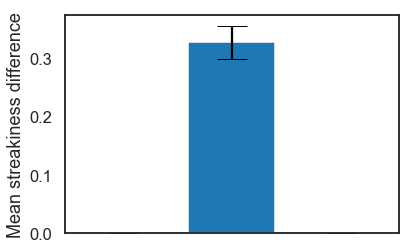
\includegraphics[width=1.2\textwidth]{figures/bird_streak_diff.png}
\caption{Bird}
\end{subfigure}
 \hfill
\begin{subfigure}[t]{0.2\textwidth}
\centering
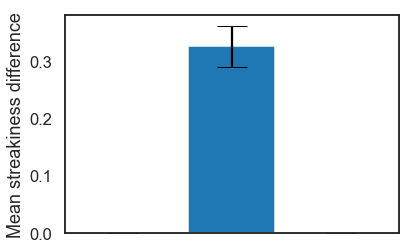
\includegraphics[width=1.2\textwidth]{figures/car_streak_diff.png}
\caption{Car}
\end{subfigure}
\hfill
\begin{subfigure}[t]{0.2\textwidth}
\centering
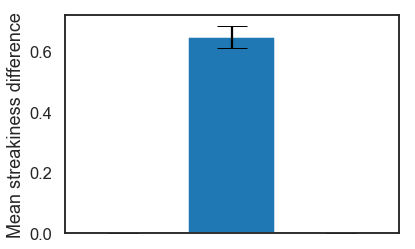
\includegraphics[width=1.2\textwidth]{figures/chair_streak_diff.png}
\caption{Chair}
\end{subfigure}
 \hfill
\begin{subfigure}[t]{0.2\textwidth}
\centering
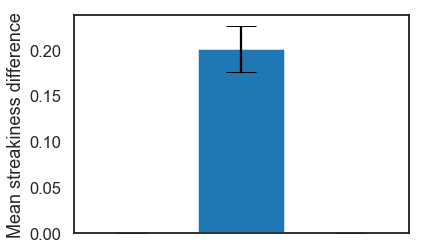
\includegraphics[width=1.2\textwidth]{figures/dog_streak_diff.png}
\caption{Dog}
\end{subfigure}
\caption{Streak length differences for each sketch category}
\end{figure}

The following are the means and standard deviations for the distributions of the difference between true and scrambled streak lengths for each of the object categories.
Bird: Mean = 0.33 , Std = 0.015
Car: Mean = 0.33, Std = 0.018
Chair: Mean = 0.65 , Std = 0.018
Dog: Mean = 0.20 , Std = 0.013


% table for now: Is there spatial contiguity in how people structure their sketches?

\subsection{Modulation between communicative contexts}
\jefan{where we would report analysis of the sketch part features (num strokes, arc length)
e.g., when the far sketches are more abstract, how does that manifest in this feature representation?
like, are they more similar to each other, more like "bird" and lacking object-specific details?
a way of measuring this is that the centroid (euclidean norm, magnitude of the vector) is closer to the origin for far vs. close, and also that the RMSD to centroid of far sketches is smaller than for close sketches.... }


\section{Discussion}

\section{Acknowledgments}

\subsection{Tables}

\subsection{Figures}






\section{References}

\bibliographystyle{apacite}

\setlength{\bibleftmargin}{.125in}
\setlength{\bibindent}{-\bibleftmargin}

\bibliography{CogSci_Template}


\end{document}
